\documentclass{beamer}
\usepackage{multicol}

\usepackage{hyperref}
\hypersetup{
	colorlinks=true,
	linkcolor=blue,    
	urlcolor=blue,
}
\usepackage{tikz}
\usetikzlibrary{shapes,arrows}
\tikzstyle{arrow} = [->,>=stealth]

\useoutertheme{infolines}
\usecolortheme{seagull}
\usefonttheme{professionalfonts}

\logo{
	
\includegraphics[width=1cm]{GUSEC.jpg}
}

\AtBeginSection[]
{
	\begin{frame}
		\frametitle{Outline of the Workshop}
		\tableofcontents[currentsection]
	\end{frame}
}


\title{\textit{Introduction to x86 Assembly}}
\author{Joe Rose}
\institute{GUSEC}
\date{\today}

\tikzstyle{block} = [rectangle, draw, fill=blue!10, 
text width=3cm, text centered, rounded corners, minimum width=3cm, minimum height=1cm]

\tikzstyle{blockhard} = [rectangle, draw, fill=blue!10, 
text width=3cm, text centered, minimum width=3cm, minimum height=1cm]

\begin{document}
	
	\frame{\titlepage}
	
	\begin{frame}{Outline of the Workshop}
		\tableofcontents
	\end{frame}
	
	\section{Introduction}
	\begin{frame}
		\frametitle{Who am I?}
		\begin{itemize}
			\item 3rd Year Comp. Sci. Student
			\item Secretary of GUSEC
			\item Big nerd
		\end{itemize}
	\end{frame}
	
	\section{System Architecture}
	
	\begin{frame}
		\frametitle{Abstraction}

		Modern computer systems can be represented as layers of \textit{abstraction}. As software engineers, we generally work in a 'high level' highly abstracted space, which is then converted by our compiler into low level \textit{machine code}. 

		\begin{center}
			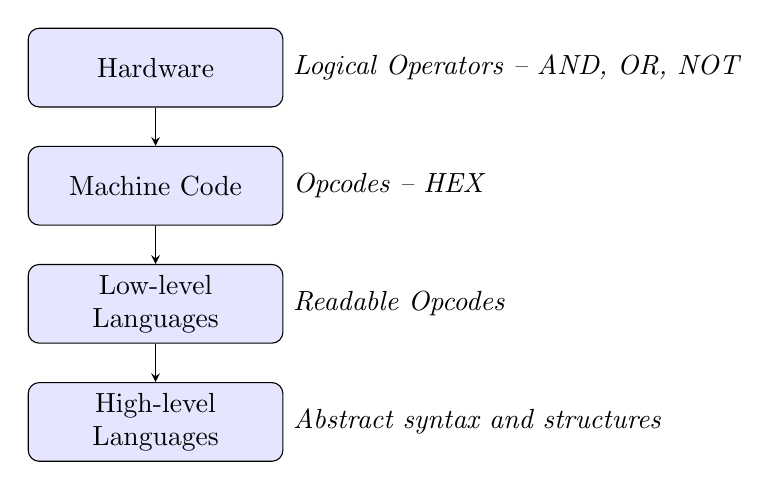
\begin{tikzpicture}[node distance = 1.5cm, auto]
				% Place nodes
				\node (hardware) [block,label=east:\textit{Logical Operators -- AND, OR, NOT}] {Hardware};
				\node (machinecode) [block, label=east:\textit{Opcodes -- HEX}, below of=hardware] {Machine Code};
				\node (lowlevel) [block, label=east:\textit{Readable Opcodes}, below of=machinecode] {Low-level Languages};
				\node (highlevel) [block, label=east:\textit{Abstract syntax and structures}, below of=lowlevel] {High-level Languages};
				
				% Draw arrows
				\draw [arrow] (hardware) -- (machinecode);
				\draw [arrow] (machinecode) -- (lowlevel);
				\draw [arrow] (lowlevel) -- (highlevel);

			\end{tikzpicture}
		\end{center}
	\end{frame}
	
	\subsection{Memory}
	
	\begin{frame}
		\frametitle{x86 Memory}
		
		Memory, as it has come to be defined in some current literature, is somewhat of an abstract concept, this is because understanding memory is \textbf{really} complex. In this workshop, we're going to be using a \textit{flat memory} model, which is basically just thinking of memory as like a Hash. Each memory location being an 8-\textbf{byte} 'bucket' which is mapped to by a 32-\textbf{bit} memory address. This allows for a possbile $2^{32}=4294967295$ possible addresses. 
		\newline
		
		As an aside, this is why 32-bit computers can only really address up to 4GiB of RAM, and FAT32 formatted USB drives can only store up to 4GiB files. 
	\end{frame}
	
	\begin{frame}
		\frametitle{Memory for a Process}
		
		Every process running at a given time is carved out a little piece of virtual memory. It follows roughly this construction
		
		\begin{center}
			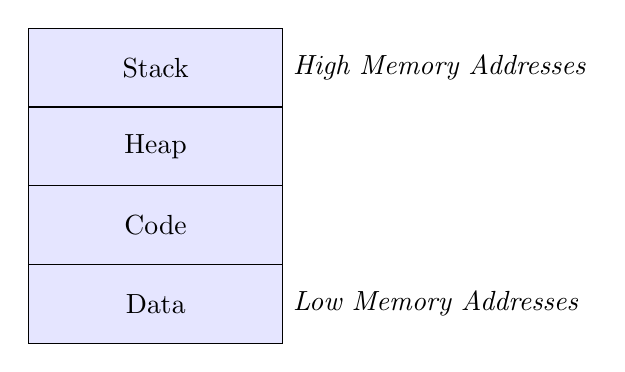
\begin{tikzpicture}[node distance = 1cm, auto]
				% Place nodes
				\node (hardware) [blockhard,label=east:\textit{High Memory Addresses}] {Stack};
				\node (machinecode) [blockhard, below of=hardware] {Heap};
				\node (lowlevel) [blockhard, below of=machinecode] {Code};
				\node (highlevel) [blockhard, label=east:\textit{Low Memory Addresses}, below of=lowlevel] {Data};
				
				
			\end{tikzpicture}
		\end{center}	
	\end{frame}
	
	\subsection{Registers and Flags}
	
	\begin{frame}
		\frametitle{The Registers}
		
		In low-level languages we deal with the regsiters. Registers are extremely small (32-\textbf{bit}) pieces of memory within your CPU which are quicker than RAM or cache to access. These are what store the pieces of data currently being worked with. The x86 specifies some general purpose registers and some dedicated registers. There are 16 registers in total, but here are some of the most important. 
		\newline
		
		\begin{tabular}{|c|l|}
			\hline
			\textbf{Register} & \textbf{Purpose} \\
			\hline
			\hline
			EAX & Accumulator\\
			\hline
			ECX & Counter in loops\\
			\hline
			ESI & Source in string \& memory operations\\
			\hline
			EDI & Destination in string \& memory operations\\
			\hline
			EBP & Stack base pointer\\
			\hline
			ESP & Stack Pointer\\
			\hline
			EFLAGS & Collection of flags \\
			\hline
		\end{tabular}
	\end{frame}
	
	\begin{frame}
		\frametitle{Flags}
		
		These are simple way of the computer keeping tracking its current state. All the flags are stored in the EFLAGS register and are set automatically when certain conditions are met. Here is a list of the most important: 
		\newline
		
		\begin{tabular}{|c|c|l|}
			\hline
			\textbf{Bit} & \textbf{Mnemonic} & \textbf{Usage} \\
			\hline
			\hline
			0 & CF & Carry Flag\\
			\hline
			2 & PF & Parity Flag\\
			\hline
			6 & ZF & Zero Flag\\
			\hline
			7 & SF & Sign Flag\\
			\hline
			11 & OF & Overflow Flag\\
			\hline
		\end{tabular}
		
	\end{frame}
	
	\section{Syntax}
	
	\begin{frame}
		\frametitle{Data Types}
		
		There aren't the traditional, high level data types that we might expect from languages like C and Python. Instead, our data types consist of a certain amout of arbitrary bits:
		\newline
		
		\begin{tabular}{|l|c|}
			\hline
			\textbf{Name} & \textbf{Amount of Bits} \\
			\hline
			\hline
			Byte & 8\\
			\hline
			Word & 16\\
			\hline
			Double Word & 32\\
			\hline
			Quad Word & 64\\
			\hline
		\end{tabular}
		
	\end{frame}

	\begin{frame}
		\frametitle{Structure}
		
		We're going to be looking at the \textit{Intel} notation for assembly language, this is it's what I learned, it's the most common notation and it's (in my opinion) more clear.
		\newline
		
		\begin{multicols}{2}
			%\textbf{Intel}
			%\begin{verbatim}
			%	mov ecx, AABBCCDDh
			%	mov ecx, [eax]
			%	mov ecx, eax
			%\end{verbatim}
			
			
			%\textbf{AT\&T}
			%\begin{verbatim}
			%	movl $0xAABBCCDD, %ecx
			%	movl (%eax), %ecx
			%	movl %eax, %ecx
			%\end{verbatim}
			
		\end{multicols}
	\end{frame}
	
	\section{Finishing Off}
	
	\begin{frame}
		\frametitle{Sources}
		
		These are the books I got the content for this workshop from. However, there is a huge amount of free literature on x86 and these are by no means necessary for you to learn the ropes. 
		\newline		
		
		\begin{itemize}
			\item \href{https://www.worldcat.org/search?q=bn:9781593274306}{\textit{Practical Malware Analysis} - Chapter 4. A Crash Course in x86 Disassembly}
			\item \href{https://www.worldcat.org/search?q=bn:9781593274306}{\textit{Practical Reverse Engineering} - Chapter 1. x86 and x64}
			\item \href{https://www.wiley.com/en-gb/Practical+Reverse+Engineering:+x86,+x64,+ARM,+Windows+Kernel,+Reversing+Tools,+and+Obfuscation-p-9781118787311}{\textit{Practical Binary Analysis} - Appendix A. A Crash Course in x86 Disassembly}
			\item \href{https://eleanor.lib.gla.ac.uk/record=b2470109}{\textit{Essentials of 80x86 assembly language}}
		\end{itemize}		
	\end{frame}
	
	
\end{document}